\documentclass[a4paper]{article}
\usepackage[dutch]{babel}
\usepackage[utf8x]{inputenc}
\usepackage{amsmath,graphicx,hyperref,parskip,setspace,fancyhdr,changepage}
\usepackage[margin=1in]{geometry}
\usepackage[colorinlistoftodos]{todonotes}

\setlength{\parindent}{0mm}
\linespread{1.4}

\newcommand{\rcom}[1]{\textbf{\textcolor{red}{#1}}}

\pagestyle{fancy}

\title{Symbolische manipulatie}
\author{Rik Voorhaar(3888169) - Jan-Willem van Ittersum(3992942) - Jurre Corver(3905985)}

\begin{document}
\maketitle
\clearpage

%\begin{abstract}
%Your abstract.
%\end{abstract}

\section{Introductie}
In deze opdracht hebben we een eigen computeralgebrasysteem (CAS) ontwikkeld om symbolisch te kunnen rekenen zoals dat bijvoorbeeld in Mathematica gebeurt. Wiskundige formules worden hiervoor opgeslagen in een zogenaamde expressie-boom. Behalve dat deze representatie kan worden gebruikt om berekeningen te doen, is deze geschikt voor symbolische manipulaties, zoals optellen, vermenigvuldigen, maar ook differenti\"eren en oplossen van sommige polynoom~vergelijkingen. De code behordende bij dit project kan gevonden worden op \url{https://github.com/JurreCorver/SymbolischeManipulatie}.


\section{Theorie}
%Beschrijving van de theorie


\section{Algoritmen}
%Beschrijving van de gebruikte algoritmen, denk hierbij ook aan bijvoorbeeld de complexiteit en de gebruikte datastructuren



\section{Documentatie}
%Documentatie over het gebruik van de code
\subsection{Installatie}
Om dit programma te gebruiken zijn naast een werkende Python 3.4 distributie enkele Python packages nodig. De niet-standaard packages zijn: \texttt{numpy, pillow, scipy, tkinter}.
Verder heeft de grafische gebruikers omgeving onderstuining voor het weergeven van de output met behulp van \LaTeX. Hiervoor is dus een werkende \LaTeX~distributie vereist. Daarbij is het ook benodigd om \emph{GhostScript} geinstalleerd te hebben. Voor \emph{Windows} gebruikers is het verder specifiek vereist om de 32-bit versie van \emph{GhostScript} te gebruiken en het pad naar \texttt{gswin32c.exe} toe te voegen aan de \texttt{\%path\%} systeemvariabele.

\subsection{Grafische omgeving}
De grafische omgeving kan gebruikt worden door \texttt{tkmain.pyw} uit te voeren. Dit kan ook vanuit de command-line door \texttt{python tkmain.pyw} uit te voeren.  De verschillende componenten van de omgeving zullen worden uitgelegd met referentie naar figuur \ref{fig:screenshot}

\begin{figure}[!htb]
  \centering
  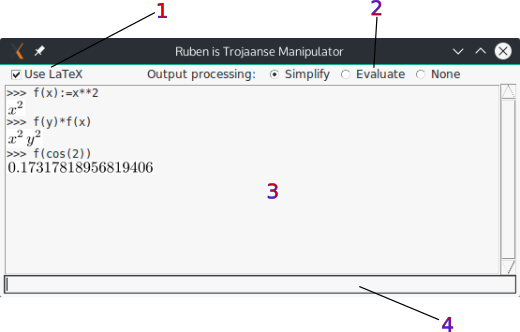
\includegraphics[width=0.6\textwidth]{screenshot.png}
  \caption{Screenshot van de grafische omgeving}
  \label{fig:screenshot}
\end{figure}

\begin{enumerate}
\item Met de \texttt{Use LaTeX} wordt gespecificeerd of de output door \LaTeX wordt verwerkt voor dat deze wordt weergegeven. Indien deze optie niet geselecteerd is zal de output als plain-text worden weergegeven.
\item De \texttt{Output processing} optie specificeerd hoe de input wordt verwerkt. Indien \texttt{Simplify} is aangevinkt zal de expressie zo veel mogelijk versimpeld worden. Terwijl bij het aanvinken van \texttt{Evaluate} de expressie wordt uitgerekend indien deze numeriek is, en anders onversimpeld wordt weergegeven. Als laatste zorgt de \texttt{None} optie juist dat de expressie niet wordt berekend en direct wordt weergegeven.
\item Dit is het scherm waar de output wordt weergegeven. Hier wordt de input van de gebruiker met \texttt{>>>} er voor weergegeven, en telkens op de regel daarna de output bij de regel input erboven. Indien er fouten optraden tijdens het uitvoeren van de input wordt dit hier ook weergegeven.
\item In dit scherm kan de gebruiker zijn input invoeren. Als de gebruiker de \texttt{Enter} toets indrukt wordt de input ge\"evaluaeerd. De pijltjestoetsen naar boven en onder kunnen worden gebruikt om de vorige input nog een keer te gebruiken.
\end{enumerate}

\subsection{Syntax}
De invoer ondersteund standaard operaties op getallen die met symbolen \texttt{*, +, -, **, /, \%} kunnen worden ingevoerd. Verder kunnen ronde haaken \texttt{( )} worden gebruikt. Enkele voorbeelden:
\begin{adjustwidth}{1.5cm}{}
\setstretch{1}
\texttt{>>> 2+2-1}\\
$1$\\
\texttt{>>> (2**3)/2}\\
$4$\\
\texttt{>>> 7 \% 3}\\
$1$
\end{adjustwidth}
Ook zijn de standaardfuncties \texttt{sin, cos, tan, arcsin, arccos, ln, exp, floor, gamma, polygamma} ge\"implementeerd. \rcom{iets meer over schrijven, voorbeeld toevoegen, log toevoegen met twee argumenten}

\rcom{dingen over == en := toevoegen, complexe getallen}

\subsection{Lijst van commando's}
\rcom{Rik: exit(), pi, e, phi, d}

\textbf{solvePolynomial(eq, var)}



\section{Resultaten}
%Eventuele resultate die behaald zijn met de code

\section{Taakverdeling}
%De taakverdeling binnen je groepje.





\begin{thebibliography}{99}

\bibitem{c1} Wikipedia - Shunting-yard algorithm:
\url{https://en.wikipedia.org/wiki/Shunting-yard_algorithm}. 
 - geraadpleegd op 28 juni 2015

\end{thebibliography}



\end{document}